\documentclass[referee,lineno,pdflatex,sn-vancouver-num]{sn-jnl}

\usepackage{graphicx}
\usepackage{url}
\graphicspath{{figures/}{./}}
\usepackage{amsmath,amssymb}
\usepackage{booktabs}
\usepackage{placeins}
\raggedbottom

\begin{document}

\title[Simulation of knee-angle prediction]{Toward the use of simulated
environments to evaluate sEMG-informed knee-angle prediction: RMSE predicts
simulated walking instability only above a threshold accuracy}

\author*[1]{\fnm{Aaron} \sur{Xiong}}
\affil*[1]{\orgname{Spring Branch Academic Institute}, \city{Houston}, \state{Texas}, \country{United States}}
\email{aaxiong2008@gmail.com}

\abstract{\textbf{Background:} Root-mean-square error (RMSE) measures the numerical
accuracy of knee-angle prediction, but it does not establish that the remaining
error changes whole-body motion. Whether a lower value corresponds to more stable
walking has not been tested.

\textbf{Methods:} A prespecified residual-fusion model was evaluated on level
walking from 90 healthy participants in Gait120.
The model predicted knee angle 100~ms ahead from knee-angle history, with surface
electromyography (sEMG) estimating a correction to the kinematic forecast. Three
surrogate sEMG conditions, which preserve the signal's statistics but destroy its
correspondence with the knee, tested whether any improvement was attributable to
sEMG content rather than to added model capacity. The predicted trajectory was
then the tracking target of a proportional-derivative override on the right knee
of a MuJoCo humanoid, against a paired unmodified reference on the same matched
MoCapAct motion. Because the fitted model converges to a narrow error band, the
same fixed panel of 80 windows was replayed at
14 checkpoints sampled along the model's
gradient-descent training path.

\textbf{Results:} Mean participant RMSE was
4.748$^{\circ}$ with residual fusion
against 5.093$^{\circ}$ without sEMG
($t(89)=7.39$, $p=7.50\times10^{-11}$;
70 of 90
participants improved).

Relating accuracy to simulated outcome across 14
accuracy levels on the same fixed panel, RMSE and
excess instability were not monotonically related over the sampled range
($\rho=+0.327$,
$p=0.253$). An exploratory two-segment split, placed between adjacent
levels, falls at 12.97$^{\circ}$ (95\% CI
12.00 to 14.24$^{\circ}$). Above it, worse prediction
gave more instability (slope
+0.01304~s per
degree, 95\% CI 0.01005 to 0.01696). Below it
the relationship inverted
(slope
-0.00707, 95\% CI
-0.00967 to -0.00467).

\textbf{Conclusions:} Prediction RMSE tracked the simulated walking outcome
above roughly 13$^{\circ}$ and inverted
below it, so a lower value does not indicate a more stable simulated gait
across the whole range. The inversion arises because a partially fitted model regresses
toward the participant mean and so commands a flatter trajectory that moves the
knee less than the recorded motion does. A converged predictor therefore sits in
the regime where lower RMSE no longer implies better simulated behavior. The
sEMG correction itself, which improved prediction, did not detectably change the
simulated outcome (+0.0084~s, 95\% CI
-0.0032 to 0.0199; $p=0.153$).}

\keywords{surface electromyography, knee-angle prediction, prosthetic control,
biomechanics, MuJoCo, motion matching, extrapolated center of mass}

\maketitle

\section{Introduction}\label{sec:introduction}
Lower-limb amputation remains a substantial rehabilitation problem in the United States, and transfemoral (above-the-knee) amputation is especially disruptive because it removes the knee joint and many of the mechanical advantages that it provides during standing, walking, sitting, and transitions onto different terrain \cite{dillingham2002,pran2021}. Even with contemporary microprocessor-based artificial knees, users frequently walk more slowly, expend more mechanical work, and experience functional limitations that can vary from one wearer to another \cite{pinhey2022}. Following from these limitations of the status quo, the main goal of current research continues to be the accurate reconstruction of the knee trajectory across changing gait states, variable sensor conditions, and differences in movement and body structure from patient to patient.

The major challenge in transfemoral prosthetics is that direct information about the missing or mechanically replaced joint is unavailable to predictive solutions for the knee angle. A reconstructive algorithm must instead infer knee behavior from nearby available signals that are practical and preferably non-invasive to collect from the patient. Surface electromyography (sEMG) provides a window into muscle activations, while inertial measurement units (IMUs) give predictor models kinematic information from the limbs, such as acceleration, angular velocity, and position \cite{deluca1997,farina2014}. These signals are valuable for different reasons. sEMG contains neuromuscular intent, but is noisy, non-stationary, and sensitive to fatigue, variance in electrode placement, skin impedance, and inter-subject variability, which is why artificial intelligence and machine learning techniques are commonly used to process this rather volatile signal \cite{huang2008,chowdhury2013,phinyomark2018}. IMUs are comparatively stable, but encode the current physical state of the limbs and body rather than the direct intent of a patient to activate a specific muscle group. The task of prediction, or regression, as it is referred to in the literature, involves fusing the noisy sEMG signal with contextual kinematic data from IMUs to estimate the knee angle at some future horizon, typically tens to hundreds of milliseconds from the time the sEMG and IMU data are captured.

\subsection{Current methods for knee-angle prediction}
This major inference problem has been studied with both classical and deep methods in machine learning. Earlier work in myoelectric control relied heavily on feature-engineered models and pattern-recognition pipelines, including support vector methods, relevance vector regression, and handcrafted EMG features \cite{hudgins1993,hargrove2007,lihb2023}. More recent studies show that convolutional neural networks (CNNs) and long short-term memory networks (LSTMs) can model time dependencies in continuous joint-angle prediction more effectively than many classical benchmarks, particularly when sEMG and kinematic information are combined into a temporally aware model \cite{sun2022,yi2022,zhang2022,zhu2022,moghadam2023,keles2023}. Transformer-based models have also shown strong results in wearable biomechanics and myoelectric prediction, particularly when sequence length and cross-subject generalization become central concerns \cite{zerveas2021,liang2023,lix2023,linhe2024,lin2025a,mollahossein2025}. At the same time, systematic reviews of EMG-driven lower-limb prosthetic control still describe the field as methodologically evolving, with researchers trying novel techniques, especially with respect to preprocessing, validation strategy, and model architecture, to improve on current benchmarks \cite{cimolato2022,ahkami2023}.

\subsection{Simulation of virtual prosthetics}
The primary problem with the current evaluation metric, cross-validation Root Mean Squared Error (RMSE), is that prediction accuracy alone does not guarantee the prosthetic's true usefulness in an actual kinematic context. Joint-angle regressors, such as the methods described above, are only valuable if their outputs are biomechanically plausible when considered in the context of whole-body motion. This gap between statistical error and real-time function has already been examined in myoelectric control research. Hargrove et al.\ \cite{hargrove2007}, for example, evaluated a pattern-recognition controller through a real-time virtual environment rather than solely reporting classifier accuracy. Similarly, Krasoulis et al.\ \cite{krasoulis2019} showed that prosthetic finger performance improved with user practice and could not be reliably inferred from machine learning statistics alone. Together, these studies suggest that a low RMSE could hide functionally poor control of the prosthetic.

Another issue is that real human-subject testing is difficult, expensive, and potentially risky. Testing a weak or unstable controller on an actual prosthesis could create safety concerns for the user. For that reason, virtual environments and physics-based simulation can serve as an intermediate evaluation layer between offline prediction and real-world trials.

Physics-based simulation offers a closer approximation to a real-life locomotion context because it models bodies using joints, forces, contacts, and dynamics instead of simply displaying a motion visually. One Python implementation of physics-based simulation is MuJoCo, a physics engine commonly used in research for model-based control and simulated articulated bodies \cite{todorov2012}. For prosthetic research, this kind of engine is valuable because it can test whether a predicted movement is dynamically plausible in a controlled environment. A simulated body can fall, lose balance, or react poorly to a control signal, which provides information that a static prediction-error number cannot provide.

Motion-capture-based resources also help make simulation more realistic. MoCapAct provides motion-capture-based humanoid control data, allowing simulated movement to be grounded in recorded human-like motion rather than arbitrary synthetic poses \cite{wagener2022}. One derivative technique is motion matching, a related idea from video game character animation in which a system searches a database for the motion clip that best matches a query \cite{clavet2016}. In a prosthetic-evaluation setting, motion matching is useful because it can place a predicted joint trajectory into a broader whole-body movement context. Without that context, a knee prediction remains only a time-series output; with context, it can be examined as part of a simulated gait sequence.

It is important to note that simulation is not a replacement for real human testing. A simulated body is still a simplified model of a real person, and simulated instability is not the same as a clinical fall outcome. However, simulation can still expose a gap between local prediction accuracy and whole-body functional behavior. A model that performs well by RMSE may produce a trajectory that is poorly timed, physically awkward, or destabilizing once inserted into a locomotion system. Conversely, a slightly higher-RMSE trajectory may not be physically harmful if its errors occur in less sensitive parts of the gait cycle. Going forward, simulation offers a way to evaluate joint-angle prediction by its effect on movement rather than by prediction error alone.

\subsection{Balance metrics and functional evaluation}
A common method of physically evaluating locomotion behavior is to assess the balance of a full-body system during a walk cycle. This is traditionally done by finding the center of mass, or CoM, which constitutes the average position of the mass distributed across the body. During standing, keeping the CoM over the feet is closely related to staying balanced and upright. In a moving scenario, however, determining instability is more complex. A person's CoM may be in an acceptable position at one instant but still moving quickly enough that a corrective step is needed lest a loss of balance occur. The extrapolated center of mass, or XCoM, accounts for this by incorporating both the CoM and its velocity, allowing dynamic movement to be represented while examining balance \cite{hof2005,hof2008}.

To determine whether the XCoM is in an acceptable state, an area called the support polygon must be defined. In double support, or two-legged motion, the support polygon includes the area between both feet. The relationship between the XCoM and the support polygon is defined by a metric called the support margin; if the XCoM remains within the support polygon the margin is positive, and the body is generally easier to stabilize. If the XCoM strays too far, corrective steps by the legs may be necessary to prevent falling, resulting in high instability (i.e., stumbling) \cite{hof2005,hof2008}.

Functional evaluation in prosthetics research thus requires more than numerical predictive accuracy. Equally important to consider, if not more so, is the question of whether or not the knee angle derived from the prediction model remains compatible with gait, support, and balance in a full physical context. The literature has made strong progress improving on current numerical benchmarks, but a remaining gap can be found by questioning if those numerical benchmarks are accurate representations of functional success. RMSE can show that a model reconstructs a target angle accurately, but it cannot by itself show whether that angle would preserve the balance and the characteristics of the original motion as part of a physical system. This gap motivates simulation-based evaluation as the next step in assessing prosthetic regression models.

Two features of how such evaluations are ordinarily built stand in the way of
testing directly whether prediction accuracy corresponds to functional behavior. The first concerns where the predictor sits. Hargrove et
al.\ \cite{hargrove2007} drew a distinction between offline scoring and
real-time control, and the same distinction applies to simulation: a rollout that
reproduces a recorded error by displacing a reference trajectory has to be handed
the recorded future target in order to do so, and a controller supplied with the
answer is replaying a recording rather than controlling. Only a predictor placed inside the
control loop, generating the signal that the simulated joint actually follows,
tests what a deployed model would do. The second concerns the range of accuracy
examined. A converged model occupies a narrow band of error, and an association
estimated inside that band cannot separate the possibility that error does not
matter from the possibility that error did not vary. A study that evaluates one
trained model can only compare prediction windows against one another, where
differences are dominated by which motion each window contains rather than by the
predictor that drove it.

The present study addresses the question by holding the evaluation panel fixed and
varying the model instead. One fixed panel of walking windows is replayed at a
series of accuracy levels sampled along a single model's own gradient-descent
training path, with the predicted knee angle serving as the tracking target of the
simulated joint throughout. Because the windows, the matched reference motions,
and the initial states are identical at every level, the only thing that differs
between them is the model. That makes it possible to ask whether
RMSE and simulated walking instability are related at all, and if so, across which
part of the accuracy range.


\begin{figure}[!htbp]
\centering
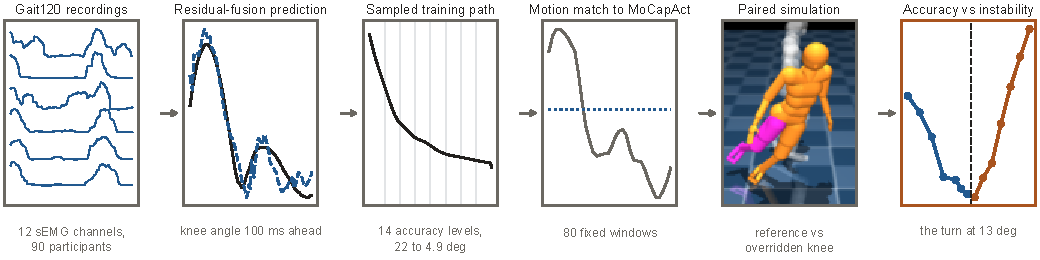
\includegraphics[width=\linewidth]{fig01_overview}
\caption{Overview of the experiment. The same fixed panel of one-second windows is replayed at every accuracy level, so window identity, matched reference motion, and initial state are held constant.}\label{fig:overview}
\end{figure}

\section{Methods}\label{sec:methods}

\subsection{Data preparation}

The experiment used the public Gait120 dataset, which contains synchronized
full-body kinematics and right-leg sEMG from 120 healthy adult men performing
seven movement tasks \cite{boo2025,boo2025dataset}. Only level walking was used, so
that every prediction window the panel draws on comes from walking on the
level.

Participants S001--S030 formed a development cohort used to choose
hyperparameters. The reported experiment used the remaining
$n=90$ participants, S031--S120, referred to below
as the confirmation cohort. Within each
participant, trials 1--3 were used to fit the model and to compute the mean and
standard deviation of that participant's twelve sEMG channels and knee angle,
which standardize the inputs and the target. Trial 4 was reserved for checking
the fit and is not reported. Trial 5 was held out and used
for neither purpose, and is the trial every reported number comes from.

Each participant contributed one value to every analysis: the mean error over
that participant's trial 5 \cite{roberts2017}.

The released sEMG was sampled at 2000~Hz and the OpenSim joint angles at 100~Hz.
Twelve right-leg sEMG channels were retained. Each was filtered with
a second-order 20--500-Hz Butterworth band-pass, rectified, and converted to a
causal 250-sample (125-ms) root-mean-square envelope
\cite{chowdhury2013,phinyomark2018}. No future sEMG entered an input frame.
Predictor inputs and targets were not interpolated or time-normalized.

\subsection{Windowing, forecast horizon, and training}

Each prediction example contained 60 knee-angle frames (600~ms) and the final 15
sampled envelope frames (150~ms) from all 12 sEMG channels. The target was the
recorded knee angle 100~ms after the final input frame. That horizon is longer
than the electromechanical delay between muscle activation and the resulting
joint movement \cite{cavanagh1979}, so an sEMG sample can carry information
about motion that has not yet happened, and it matches the horizon at which
comparable work predicts future knee angle from myoelectric and kinematic
signals \cite{coker2021}.

The design places two requirements on the predictor. The first is that the model's accuracy can be varied
continuously across a wide range and returned to the same endpoint every time,
which is what locating the turn depends on. A convex objective with a closed-form
solution gives that: descent runs from the participant mean to the exact analytic
optimum, and that optimum is the terminal checkpoint rather than an approximation
of it. The second is that the sEMG contribution can be removed exactly, because setting the correction to zero removes the signal
from a model that has already been fitted, instead of requiring a second fit whose
capacity and initialization would differ. A convolutional, recurrent, or
transformer predictor of the kind reviewed above would follow a stochastic
training path to an endpoint that is not exactly reproducible, and its ablation
would confound signal content with model capacity.

One participant-balanced pair of ridge regressions was fitted to trials 1--3
\cite{hoerl1970}. The first predicted standardized future knee angle from the
60-frame knee history. The second predicted the remaining training residual from
the sEMG history. Equal total weight per participant prevented participants with
more eligible frames from dominating the fit. The fused estimate was

\begin{equation}
\hat y_{\mathrm{fusion}}=\hat y_{\mathrm{kin}}+\gamma c_{\mathrm{EMG}},
\label{eq:fusion}
\end{equation}

where $\hat y_{\mathrm{kin}}$ was the kinematic forecast and $c_{\mathrm{EMG}}$ the
estimated residual correction. The comparison without sEMG used the same fitted
kinematic stage with $c_{\mathrm{EMG}}=0$. Ridge penalties selected on the
development cohort were 0.1 for the kinematic stage
and 10.0 for the residual stage, with
$\gamma=1.0$. The residual output was bounded as
$b\tanh(c_{\mathrm{EMG}}/b)$, where $b$ was each participant's 95th percentile
absolute kinematic residual from trials 1--3.

\subsection{Attributing the improvement to sEMG}

Because penalties were fixed on a separate development cohort and every model was
scored on a later trial that no fit had seen, added capacity that
fitted noise would raise held-out error rather than lower it. As a
further check, three surrogate conditions repeated the whole confirmation fit with
the sEMG replaced by a signal preserving its statistics but not its correspondence
with the knee; these are reported in the supplementary analysis of surrogate
controls. Every paired
comparison was tested with a two-sided paired $t$-test on the per-participant
differences.

A separate timing control shifted the same sEMG history 500~ms earlier within each
continuous trial, evaluating aligned and shifted models on identical target rows.


\begin{figure}[!htbp]
\centering
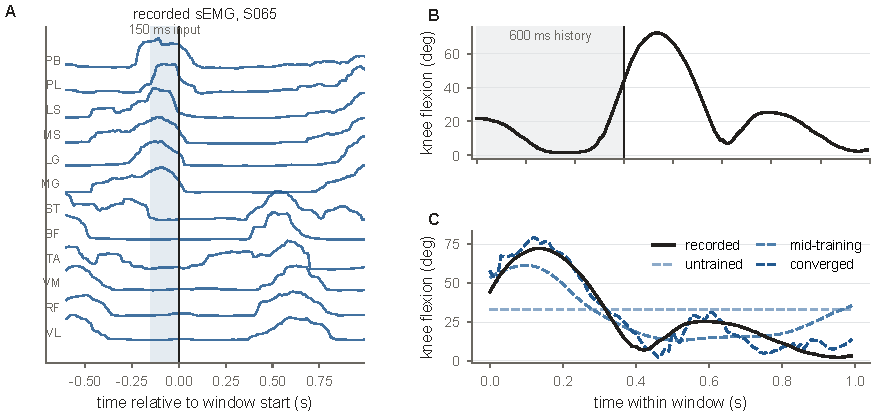
\includegraphics[width=\linewidth]{fig02_signals}
\caption{Recorded signals and predictions for one panel window. \textbf{A} The twelve recorded right-leg sEMG envelopes, standardized, with the 150~ms input interval shaded. \textbf{B} The recorded knee trajectory, with the 600~ms history interval shaded. \textbf{C} The recorded knee against predictions from three points on the training path. The untrained model predicts close to the participant mean, mid-training predictions are smoothed relative to the recording, and the converged model tracks it closely.}\label{fig:signals}
\end{figure}

\subsection{Sampling a range of prediction accuracy}

The residual-fusion model has a closed-form solution, which yields one converged
model and no trajectory to sample. Refitting on nested fractions of the
trial 1--3 fitting data does not help: a linear model fitted to a small fraction of
90 participants' level walking is already close to its converged error, so every such
checkpoint lands in the same narrow band.

Instead, the same model class was fitted by full-batch gradient descent on the same
participant-balanced ridge objective, from a zero coefficient vector. At step zero
each stage predicts the participant-balanced target mean, so the path begins with an error close to the
standard deviation of the knee angle itself and descends to the closed-form
solution,
which is appended as the terminal checkpoint. The descent therefore ends on exactly
the model the confirmation run reports rather than near it.

The step size was set well below the largest value for which the descent still
converges. The reason is sampling resolution rather than stability: near that
value the first steps collapse most of the error, so the high-error region is crossed between recorded points and cannot
be sampled. Checkpoints were placed to tile the achieved training-RMSE range
rather than the step index, because descent spends most of its steps near
convergence. The reported path ran 400,000 steps and
spanned 22.00$^{\circ}$ to
4.94$^{\circ}$ training RMSE across
14 checkpoints.


\subsection{Motion matching and physics evaluation}

The fixed physics panel was drawn from confirmation trial 5 before matching or
simulation outcomes were known. A seeded participant-balanced procedure selected
80 one-second windows, giving each eligible participant one
window before assigning a second, so the panel draws on
65 participants, of whom 15 contribute two
windows. Prediction error was not used for selection. Windows are therefore
nested within participants, which the bootstrap over accuracy levels takes into
account.

Each query was matched against the whole MoCapAct expert bank
\cite{wagener2022}, which supplies short motion-capture clips, termed snippets,
and for each one a policy trained to reproduce that clip in simulation, termed
its expert policy. No motion label restricted the candidates, since the released
snippets carry none; a match was selected on knee-trajectory agreement alone,
and the agreement achieved is reported below and carried as a covariate. Candidate snippets were aligned by a constant knee offset and
either sign convention, without amplitude scaling. Knee RMSE determined the match
rank; the RMS geodesic angle between the query and candidate right-thigh
orientations was retained as a match-quality covariate. Mean
matching knee error was 3.78$^{\circ}$
(median 3.44$^{\circ}$) and mean thigh
orientation RMS 4.10$^{\circ}$.

In the prediction condition the model's predicted knee angle was the tracking
target of a proportional-derivative override on the right knee actuator. The
prediction was first mapped into the matched clip's convention using the constant
offset and sign that the match established:

\begin{equation}
\tau=K_p(q_{\mathrm{des}}-q)+K_d(\dot q_{\mathrm{des}}-\dot q),
\qquad q_{\mathrm{des}}(t)=\hat y(t).
\label{eq:control}
\end{equation}

Proportional and derivative gains were $K_p=400$ and $K_d=20$ with the actuator
force limited to 160, and the desired velocity was the causal backward difference
of the commanded trajectory, zero at the first evaluation step. The gains were
set by requiring that commanding a matched clip's own recorded trajectory
reproduce that trajectory in joint space to within
10$^{\circ}$; no prediction was used to
set them.

The paired reference condition ran the unmodified expert policy on the same
snippet, initial state, and controller, and began from the same point in the
clip after the same number of warm-up steps, which are simulation steps run
before the evaluation window so that the policy is already tracking the clip
when measurement starts. Nothing in either rollout reads
the recorded future knee angle, so the simulation is driven by the model output
rather than by a replayed error.



\begin{figure}[!htbp]
\centering
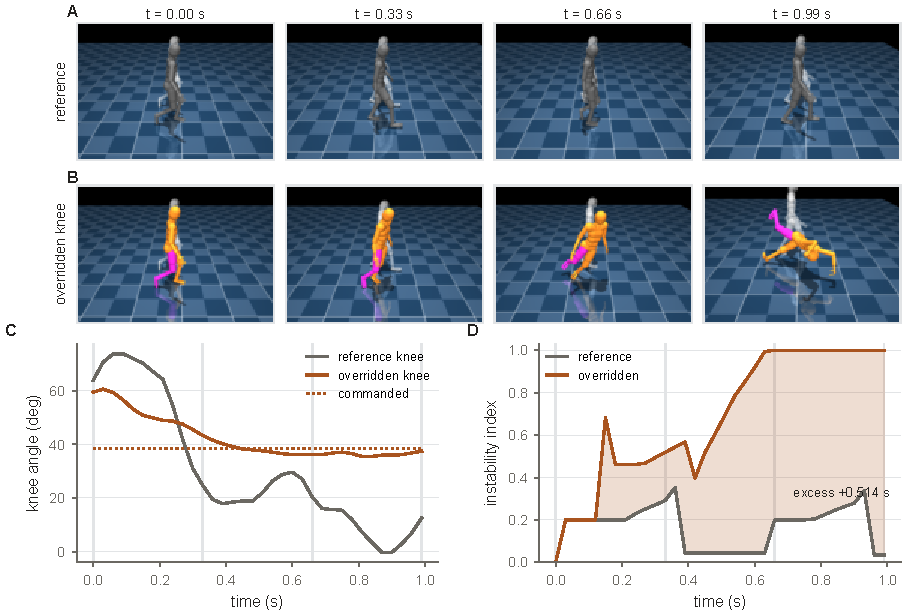
\includegraphics[width=\linewidth]{fig04_simulation}
\caption{A paired rollout at the least accurate model. \textbf{A} The unmodified reference. \textbf{B} The same matched motion with the right knee overridden; the substituted shank is highlighted. \textbf{C} Realized and commanded knee angle in both conditions. \textbf{D} The instability index in both conditions; shading marks the excess instability that is integrated to give the outcome.}\label{fig:simulation}
\end{figure}

\subsection{Evaluating simulations with an instability metric}

At each control step the convex hull of foot--ground contact points defined the
support polygon, and the XCoM extrapolated the horizontal center-of-mass
position in the direction of its velocity. Let $m$ be the signed distance from the
XCoM to the boundary of that polygon, in meters, positive when the XCoM lies
inside it.

The instability index was computed at each step from the trailing ten control
steps of $m$. Writing $m_{\mathrm{min}}$ and $m_{\mathrm{end}}$ for the
smallest and the last margin in that window, and $s$ for the slope of $m$ across
it in meters per second, three terms were each clipped to $[0,1]$,
\begin{equation}
r_{\mathrm{min}}=\frac{-m_{\mathrm{min}}-0.42}{0.40},\qquad
r_{\mathrm{end}}=\frac{-m_{\mathrm{end}}-0.30}{0.35},\qquad
r_{s}=\frac{-s-0.15}{0.45},
\end{equation}
and combined into the index
$I=0.55\,r_{\mathrm{min}}+0.25\,r_{\mathrm{end}}+0.20\,r_{s}$, again
clipped to $[0,1]$. Each term is zero while the XCoM stays near or inside the
support polygon and reaches one when it is far outside it or leaving it quickly.
The ramp endpoints and weights were set on reference walking and running so that
unperturbed motion scores near zero. Steps at which no support margin could be
computed, such as flight phases, were given $I=0.25$.

Integrating $I$ over the window gives a quantity in seconds. Absolute instability depends on how stable a
matched reference already is,
so the reported outcome is excess instability, $I'=I_{\mathrm{PRED}}-I_{\mathrm{REF}}$,
measured against each window's own paired reference. The index is derived from
the XCoM margin, is specific to this study, and has not been validated as a
clinical stability or fall-risk measure. It falls whenever the commanded
trajectory perturbs the body less, which a trajectory that moves the knee less
than the recording also does, so a smoother or flatter command scores well
without necessarily being better gait.

\subsection{Correlation study}

The primary association was a partial Spearman correlation between window
prediction RMSE and excess instability, controlling for matching knee RMSE and
thigh orientation RMS, following Frisch--Waugh--Lovell residualization on ranked
variables \cite{spearman1904,frisch1933,lovell1963}, and is called the
match-adjusted association below.

Three complementary analyses are reported. \emph{Per checkpoint} repeats that analysis at each
accuracy level and carries the RMSE spread available to it, which separates a
near-zero association from a near-zero spread.
\emph{Within window} correlates each window's own accuracy against its own excess
instability across checkpoints and combines results with a Fisher-$z$ one-sample
test, which removes matched motion, snippet, and initial state as sources of
variation. \emph{Pooled} uses every checkpoint--window pair with a window-level
cluster bootstrap, since each window recurs once per checkpoint.

The two-segment description of the accuracy--instability curve was not
prespecified. It was chosen after plotting the checkpoint means, on seeing that
a single monotone coefficient did not describe them, and is therefore
exploratory: it reports where the sampled association changes sign rather than
testing a hypothesis fixed in advance. Its split is found by trying every
position between adjacent levels and keeping the one with the smallest combined
residual sum of squares, and its interval comes from a bootstrap that resamples
participants and carries each drawn participant across every checkpoint.

\section{Results}\label{sec:results}

\subsection{Prediction accuracy}

Mean participant RMSE on the held-out trial was
4.748$^{\circ}$ with residual fusion
and 5.093$^{\circ}$ without sEMG. The
paired improvement was 0.345$^{\circ}$ (95\%
bootstrap CI 0.254 to 0.436$^{\circ}$; two-sided
paired $t(89)=7.39$, $p=7.50\times10^{-11}$), and
70 of 90
participants improved.

The timing control is computed on the
66 participants
whose trials contain a row 500~ms earlier for every target row, so the shifted
and aligned models are scored on identical data. Moving the same sEMG history
500~ms earlier changed participant RMSE by -0.085$^{\circ}$
relative to the aligned model (95\% CI
-0.202 to 0.030$^{\circ}$;
$t(65)=-1.42$, $p=0.160$). Three surrogate
controls are reported in Table~\ref{tab:controls}.
The recorded signal outperformed all three surrogates in paired within-participant comparisons (smallest margin 0.288$^{\circ}$, all $p\leq1.68\times10^{-7}$).



\begin{figure}[!htbp]
\centering
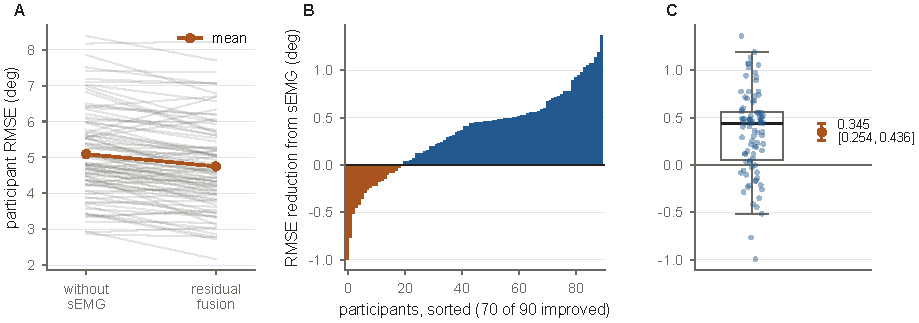
\includegraphics[width=\linewidth]{fig03_prediction_accuracy}
\caption{Prediction accuracy with and without the sEMG correction. \textbf{A} Held-out participant RMSE with and without the sEMG correction, paired within participant. \textbf{B} Per-participant RMSE reduction, sorted. \textbf{C} Distribution of the reduction with its bootstrap mean and 95\% interval.}\label{fig:accuracy}
\end{figure}

\subsection{Motion matching and paired simulation}

Across the fixed panel, the paired difference in excess instability between
the residual-fusion and no-sEMG conditions was +0.0084~s (95\% CI -0.0032 to 0.0199;
$t(79)=1.44$, $p=0.153$). The
prediction improvement attributable to sEMG was therefore not accompanied by a
detectable change in the simulated outcome.



\begin{figure}[!htbp]
\centering
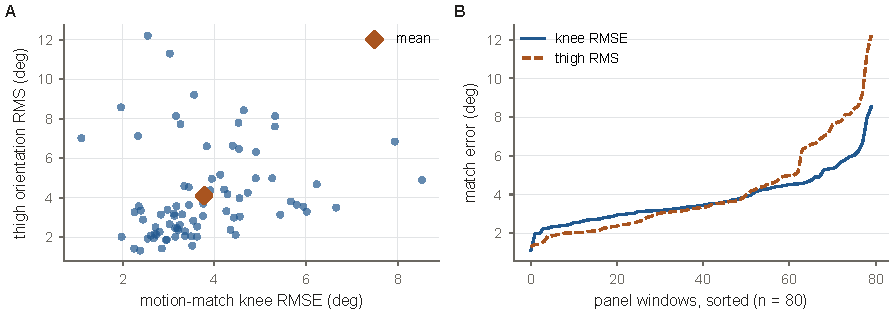
\includegraphics[width=\linewidth]{fig05_motion_matching}
\caption{Motion-match quality over the fixed panel. \textbf{A} Knee against thigh-orientation matching error for each window, with the panel mean. \textbf{B} Both errors sorted across windows.}\label{fig:matching}
\end{figure}

\subsection{Prediction error vs. excess instability}

Prediction error tracked simulated instability above a threshold accuracy,
below which the relationship reversed.

Across the 14 sampled accuracy levels, mean window
RMSE spanned 5.09$^{\circ}$ to
20.25$^{\circ}$ on the same
80 windows and the same matched references. A single monotone
coefficient over that whole range is uninformative
($\rho=+0.327$,
$p=0.253$), because the relationship is not
monotone. Searching the sampled levels for the best two-segment split places
it between adjacent levels, at
12.97$^{\circ}$ (95\% CI
12.00 to 14.24$^{\circ}$); the split can therefore
take only as many values as there are gaps between levels.

Above that accuracy, worse prediction produces more simulated instability across
the 7 levels in that segment (slope
+0.01304~s per
degree, 95\% CI 0.01005 to 0.01696).

Below it the sign inverts: models that are more accurate produce \emph{more} excess
instability across the 7 levels in that
segment (slope -0.00707,
95\% CI -0.00967 to -0.00467). Both intervals exclude
zero under a bootstrap whose draws resample participants and carry each drawn
participant's windows across every accuracy level, since the same windows are
replayed at all of them; the checkpoint means themselves are smooth by
construction, so the rank correlation across levels does not rest on fourteen
independent observations.

Commanding a matched clip's own recorded trajectory, which is the zero-error
case, gave a mean excess instability of -0.0004~s over the
10 windows of a check run before the main panel, so the
inversion is not explained by a
fixed cost of substituting the knee. A partially
fitted linear model regresses toward the participant mean, so it commands a
gentler knee trajectory than the recorded one. A gentler trajectory perturbs the
body less than the true motion does, and mean excess instability is
correspondingly negative through the middle of the range, reaching
-0.0247~s.

Three further comparisons were made. Comparing windows against one another within a
single accuracy level recovers nothing at any level
(Table~\ref{tab:checkpoints}).
Across the 80 windows, the within-window Spearman correlation between a window's own accuracy and its own excess instability averaged +0.171 (95\% CI 0.018 to 0.316; $t(79)=2.23$, $p=0.029$), with 53 of 80 windows positive. Pooled across all 1120 checkpoint--window pairs
the match-adjusted association was
+0.063 (window-level cluster bootstrap 95\% CI
-0.025 to 0.160).



\begin{figure}[!htbp]
\centering
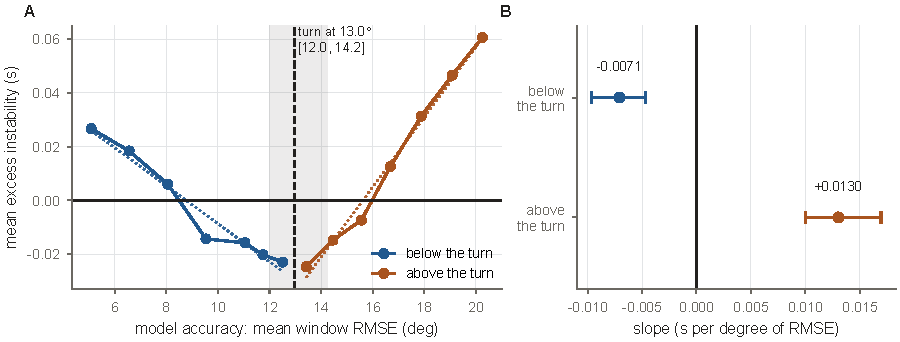
\includegraphics[width=\linewidth]{fig06_accuracy_vs_instability}
\caption{Primary result. \textbf{A} Mean excess instability against model accuracy across the sampled levels, with the fitted turn and its bootstrap interval shaded; dotted lines are the two segment fits. \textbf{B} Segment slopes with 95\% intervals from a bootstrap that resamples participants and carries each across every accuracy level.}\label{fig:primary}
\end{figure}

\begin{figure}[!htbp]
\centering
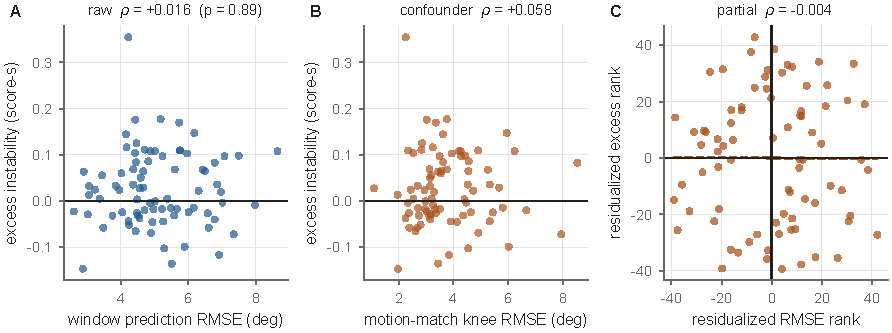
\includegraphics[width=\linewidth]{fig07_fwl}
\caption{The match-adjusted analysis at the converged model. \textbf{A} Window prediction error against excess instability. \textbf{B} The same outcome against motion-match quality, the covariate being controlled. \textbf{C} Both variables residualized on ranked match knee error and thigh orientation RMS; the correlation between them is the reported partial Spearman.}\label{fig:fwl}
\end{figure}

\begin{figure}[!htbp]
\centering
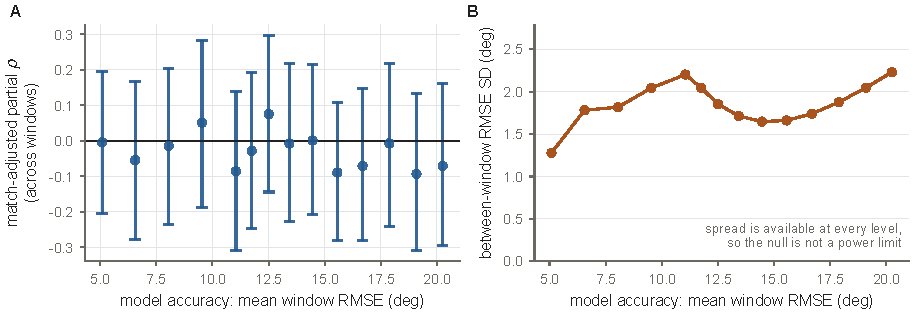
\includegraphics[width=\linewidth]{fig08_per_checkpoint}
\caption{Match-adjusted association and between-window spread at each accuracy level. \textbf{A} Match-adjusted association across windows at each accuracy level; every interval includes zero. \textbf{B} Between-window RMSE spread at each level.}\label{fig:perlevel}
\end{figure}

\begin{table}[!htbp]
\caption{Accuracy, between-window spread, and match-adjusted association at each
training-path checkpoint, ordered from the converged model to the untrained one.
Excess instability is measured against each window's own paired reference.}\label{tab:checkpoints}
\begin{tabular}{lcccccc}
\toprule
Descent step & $n$ & Mean RMSE ($^{\circ}$) & SD ($^{\circ}$) & Mean excess (s) & Partial $\rho$ & 95\% CI \\
\midrule
400001 & 80 & 5.09 & 1.28 & +0.0267 & -0.004 & -0.205 to 0.195 \\
28246 & 80 & 6.56 & 1.78 & +0.0184 & -0.054 & -0.277 to 0.167 \\
2457 & 80 & 8.05 & 1.82 & +0.0061 & -0.014 & -0.235 to 0.204 \\
521 & 80 & 9.54 & 2.04 & -0.0143 & +0.051 & -0.186 to 0.282 \\
216 & 80 & 11.05 & 2.20 & -0.0158 & -0.085 & -0.308 to 0.139 \\
106 & 80 & 11.75 & 2.05 & -0.0202 & -0.028 & -0.246 to 0.193 \\
74 & 80 & 12.51 & 1.85 & -0.0230 & +0.076 & -0.144 to 0.297 \\
55 & 80 & 13.43 & 1.71 & -0.0247 & -0.007 & -0.226 to 0.217 \\
41 & 80 & 14.46 & 1.65 & -0.0148 & +0.001 & -0.208 to 0.216 \\
30 & 80 & 15.56 & 1.66 & -0.0074 & -0.089 & -0.280 to 0.108 \\
21 & 80 & 16.69 & 1.74 & +0.0126 & -0.071 & -0.281 to 0.147 \\
13 & 80 & 17.88 & 1.87 & +0.0313 & -0.007 & -0.241 to 0.218 \\
6 & 80 & 19.09 & 2.05 & +0.0466 & -0.093 & -0.309 to 0.134 \\
0 & 80 & 20.25 & 2.23 & +0.0605 & -0.071 & -0.294 to 0.162 \\
\bottomrule
\end{tabular}
\end{table}

\section{Discussion}\label{sec:discussion}

The central finding is that prediction error and simulated walking instability are
related across the whole sampled range, with the sign of the relationship
reversing partway along it. Above
12.97$^{\circ}$ of prediction
error, a less accurate model produced a less stable simulated walker, and the
slope is positive across that region. Below that point the
relationship inverted, so that further improvements in accuracy were accompanied by
slightly more excess instability rather than less. RMSE is therefore not a general
proxy for the simulated outcome. It behaves as a proxy within a band, and the boundary
of that band falls inside the range of accuracies that contemporary models occupy.

That last point is what gives the result practical weight. The most accurate model
evaluated here reached 5.09$^{\circ}$, which
lies below the turn. Because knee-angle regression models are ordinarily compared
with one another only after convergence, the regime in which they are compared is
also the regime in which further reduction in RMSE no longer predicts a more stable
simulated gait. A study confined to that regime samples only the inverted portion of
the relationship, where lower error is accompanied by slightly more simulated
instability, so it cannot recover the positive relationship that holds above the
turn. This supplies a possible
mechanism for the more general observation, made in myoelectric control by Hargrove
et al. \cite{hargrove2007} and by Krasoulis et al. \cite{krasoulis2019}, that
offline model scores do not reliably predict functional performance. It also
suggests that the methodological evolution described in recent reviews of
EMG-driven prosthetic control \cite{cimolato2022,ahkami2023} might reasonably
extend to the evaluation stage, and not only to preprocessing, architecture, and
validation strategy.

The mechanism behind the inversion does not imply that accuracy is undesirable.
It indicates that the mapping from accuracy to whole-body behavior
is not monotone, and that the quantity being minimized during training is not the
quantity that determines stability once the prediction is placed in a body.
Moving along the training path changes the amplitude, smoothness, phase and bias
of the predicted trajectory together, and RMSE is a summary of all of them, so
what is reported here is an association along one model's path rather than an
effect of prediction error considered on its own.

The sEMG correction improved held-out prediction, and that improvement survived
three surrogate controls which preserved the signal's amplitude, spectral, and
cross-channel structure while destroying its correspondence with the knee. That is
a stronger test than an ablation alone provides, since an ablation cannot separate
signal content from the additional model capacity that accompanies it. The
predictor driving the simulations therefore draws on genuine myoelectric
information rather than on model size.

Comparisons drawn across windows and comparisons drawn within a window
give different results. Comparing windows against one another
within a single accuracy level recovers nothing at any of the
14 checkpoints, even where mean window error exceeds
20$^{\circ}$.
Between-window error spread was available at every level, ranging from
1.28
to 2.23$^{\circ}$,
and the same null appears when the outcome is normalized by rollout duration.
Comparing each window against itself does recover an association: holding the
window fixed and varying only the model, a window became more unstable as its own
prediction degraded
(+0.171,
95\% CI 0.018 to 0.316, $p=0.029$,
53 of 80 windows positive). The
difference arises because between-window variation in excess instability is
dominated by which motion a window was matched to, where in the gait cycle that
window falls, and how stable the matched reference already was. Those sources of
variation are large beside the effect of prediction error and obscure it in any
comparison drawn across windows, whereas holding the window fixed removes them.

These observations bear on benchmark design. An evaluation that varies only the
window, which is what a study
of a single converged model is restricted to, will tend to report no relationship
between prediction error and simulated outcome, not because no relationship exists
but because that contrast cannot resolve one. Varying the model along its own
training path supplies the contrast that can. Prediction error does propagate to
whole-body behavior, but the effect is small in comparison with window-to-window
variation, and a benchmark constructed from comparisons between different windows
is not a suitable instrument for detecting it.

\subsection{Limitations}

The benchmark used able-bodied level walking rather than data from transfemoral
prosthesis users, so it tests an evaluation framework on a proxy dataset, and
every participant in Gait120 is an adult man, so the cohort does not represent
the range of body structures a prosthetic controller would meet. Each
model was also fitted on earlier trials from the participant it was tested on, so
these accuracies are what a calibrated model achieves, not what a wearer would get
from a model that had never seen their data.

The kinematic stage predicts from recorded knee-angle history. A microprocessor
knee carries a joint angle encoder, so that channel would exist on a device, but
two differences separate this experiment from deployment. First, the history used
here is the trajectory of an intact biological knee, whereas a prosthetic knee
follows whatever its own controller produced; the channel is the same but its
distribution is not, so the accuracy measured here is not the accuracy a device
would achieve. Second, a deployed predictor whose output drives the knee
would receive its own past commands as input, making the kinematic stage largely
a propagator of its own trajectory. Under that arrangement the sEMG correction
becomes the only term carrying new information about the wearer's intent, so its
contribution would matter more than the held-out share reported here, not less.
Neither point is tested by this experiment, and the reported accuracy is not
comparable with methods predicting from socket-available signals alone.

The instability index has not been validated against clinical outcomes
\cite{hof2005,hof2008,curtze2024}. Simulation
outcomes also depend on motion-match quality, which is why match errors are treated
as covariates, and the conclusion holds for this evaluation
rather than for every application of the model.

Finally, the turn is located by a descriptive two-segment fit over the sampled
accuracy levels. It locates where the sampled association changes; it is not a
changepoint test with its own error rate, and the unsampled interval between
checkpoints does not define a safety threshold.

\subsection{Future work}\label{sec:future}

The turn reported here was located with one model class on one evaluation
design, and the first question for further work is whether it moves. A
predictor with a different error structure, such as a recurrent or
transformer model rather than a ridge pair, may distribute its residuals
differently across the gait cycle and place its turn elsewhere. The
training-path construction used here would locate that turn in the same way,
since it requires only a model whose accuracy can be varied continuously.

A second extension would be to move from able-bodied public recordings to data
from prosthetic users while keeping the paired reference and prediction
structure intact. That would test the framework in a setting closer to real
conditions, where the kinematic history available to the predictor is produced
by a device rather than by an intact knee, and where the distribution of that
history differs from the one used here.

Future work should also examine whether more phase-sensitive summaries of
prediction error, such as stance-weighted RMSE or error aligned to support
transitions, track simulated instability more closely than window-level RMSE
does. The present result does not show that every summary of prediction error
behaves this way. It shows that RMSE, which is the summary the field reports,
tracks simulated behavior in opposite directions either side of roughly
13$^{\circ}$.

\section{Conclusion}\label{sec:conclusion}

Replaying one fixed panel of walking windows at
14 accuracy levels sampled along a model's own
training path shows that prediction error predicts simulated walking instability
in opposite directions either side of a split in the accuracy range. Above
12.97$^{\circ}$ (95\% CI
12.00 to 14.24$^{\circ}$) a less accurate model
produced a less stable simulated walker. Below that point the relationship
inverted, because a partially fitted model regresses toward the participant mean
and so commands a flatter trajectory that moves the knee less than the recorded
motion does. Root-mean-square error therefore tracked
simulated behavior in the expected direction only above the turn, and the
converged model evaluated here,
at
5.09$^{\circ}$, sits below the turn.

The practical consequence is for how prosthetic regression models are evaluated.
Since such models are ordinarily compared after convergence, they are compared in
the regime where further reduction in error no longer predicts a more stable
simulated gait. The contrast a study chooses
matters as much as the metric: comparing prediction windows against one another,
which is all a single converged model permits, recovered no relationship at any
accuracy level, whereas comparing each window against itself across accuracy
levels did. Window-to-window variation is large enough to bury an effect that is
real but small, so a benchmark built on comparisons between windows will report no
relationship whether or not one exists.

The sEMG correction produced a small improvement in later-trial knee-angle
prediction that survived three surrogate controls, and is therefore attributable to
signal content rather than to added model capacity. The predictor evaluated in
simulation draws on genuine myoelectric information. That improvement did not
carry through to the simulated outcome: against the same panel and the same
paired references, the residual-fusion and no-sEMG conditions differed by
+0.0084~s in excess instability (95\% CI
-0.0032 to 0.0199; $p=0.153$), which is the same
point the accuracy range makes, measured directly.

\backmatter

\bmhead{Supplementary analysis: sensitivity to knee-angle input}

The kinematic stage forecasts knee angle from knee-angle history, which invites
the objection that a low RMSE mostly reflects trajectory smoothness -- the knee
predicting its own near future -- rather than information recovered from the
walker. The objection concerns what the reported accuracy measures rather than
whether the signal would be available: a microprocessor knee carries a joint
angle encoder, so knee-angle history exists at inference.

The same model was therefore refitted with the kinematic stage reading only the
surrounding body -- thigh pitch and full thigh orientation, with no channel
observing the knee -- holding the windows, horizon, ridge pair, penalties, and
trial split fixed. With the sEMG correction switched off in both, knee-angle
history gave 5.093$^{\circ}$ and
the surrounding body alone gave
5.128$^{\circ}$, a difference of
0.035$^{\circ}$.

Removing every knee-derived input therefore costs almost nothing. The information
needed to forecast the knee is already present in the surrounding kinematics, so
the knee channel is a compact carrier of it rather than a shortcut, and the
reported accuracy does not rest on the knee predicting its own future.

With sEMG active, the surrounding-body model reached
4.959$^{\circ}$ against
4.748$^{\circ}$ for knee history.
Both penalties were the ones selected for the knee-history configuration, so this
comparison is conservative toward the surrounding-body arm.

\bmhead{Supplementary analysis: sEMG surrogate controls}

The reported ablation removes the sEMG correction from a model whose penalties
were fixed on a separate development cohort and whose scores come from a held-out
later trial that no fit had seen. Under that design, extra fitted capacity
raises held-out error rather than lowering it, so the comparison already speaks to
sEMG rather than to model size. The surrogates below are a further check against
subtler possibilities, such as an sEMG channel correlating with the target through
the recording setup rather than through physiology.

Each surrogate repeats the entire confirmation fit with the sEMG replaced by a
signal that preserves its statistics but not its correspondence with the knee.
\emph{Circular shift} rotates each participant-trial sEMG block against its own
kinematics, preserving amplitudes, spectra, and cross-channel structure.
\emph{Participant swap} gives each participant another participant's sEMG.
\emph{Phase randomization} replaces each channel with a surrogate of identical
power spectrum and randomized Fourier phases \cite{theiler1992}. The kinematic
stage is shared across all four conditions, so any difference between them is
attributable to sEMG content alone.

The circular-shift surrogate retained
0.17 of the recorded
effect, which is expected rather than anomalous. Walking is periodic with a cycle
close to one second, so rotating a block of sEMG against its own kinematics cannot
remove the correspondence entirely: whatever offset the rotation lands on is still
a phase of the same repeating gait cycle. A surrogate of this kind sets a floor,
not a zero, and its residual effect quantifies how much of the apparent sEMG
benefit is recoverable from gait periodicity alone. The two surrogates that break
the correspondence without relying on a time offset both returned effects
indistinguishable from zero.

Attribution is therefore judged by a paired within-participant contrast -- whether
the recorded signal beats each surrogate for the same participant -- rather than
by whether each surrogate independently fails a significance threshold, which a
periodic-signal surrogate cannot be expected to do. The recorded signal outperformed all three surrogates in paired within-participant comparisons (smallest margin 0.288$^{\circ}$, all $p\leq1.68\times10^{-7}$).

\begin{table}[!htbp]
\caption{sEMG ablation and its surrogate negative controls. Improvement is the
participant-level reduction in held-out RMSE relative to the same fitted kinematic
stage without a correction; positive favors the correction. Share is each
surrogate's effect as a fraction of the recorded one. The final column is the
paired within-participant margin by which the recorded signal beats that
surrogate. The reported $p$-values are two-sided paired $t$-tests on per-participant
differences.}\label{tab:controls}
\setlength{\tabcolsep}{2.5pt}
\begin{tabular}{lccccc}
\toprule
Condition & Improvement ($^{\circ}$) & 95\% CI & $p$ & Share & Margin ($^{\circ}$) \\
\midrule
Recorded sEMG & +0.345 & 0.254 to 0.436 & $7.50\times10^{-11}$ & --- & --- \\
Circular shift & +0.058 & 0.005 to 0.113 & $0.041$ & 0.17 & +0.288 \\
Participant swap & -0.011 & -0.048 to 0.026 & $0.556$ & -0.03 & +0.357 \\
Phase randomized & -0.022 & -0.055 to 0.008 & $0.167$ & -0.07 & +0.368 \\
\bottomrule
\end{tabular}
\end{table}

\bmhead{Ethics approval and consent to participate}
This work is a secondary analysis of publicly available, de-identified
recordings and did not involve new human participants, so ethics approval was
not required. The original Gait120 recordings were approved by the
Institutional Review Board of the Korea Advanced Institute of Science and
Technology (KH2023-053), with written informed consent obtained from every
participant and permission to share the anonymized data publicly
\cite{boo2025}.

\bmhead{Consent for publication}
Not applicable.

\bmhead{Competing interests}
The author declares no competing interests.

\bmhead{Funding}
The author received no financial support for the research, authorship, or
publication of this article.

\bmhead{Authors' contributions}
A.X. is the sole author. A.X. designed the study, wrote the prediction,
simulation, and analysis code, carried out the analysis, interpreted the
results, and wrote the manuscript.

\bmhead{Acknowledgements}
Not applicable.

\bmhead{Data availability}
Gait120 is available at \url{https://doi.org/10.6084/m9.figshare.27677016}
\cite{boo2025dataset}. MoCapAct is available from its published release
\cite{wagener2022}.

\bmhead{Code availability}
The analysis code and the manuscript generator that produced every number in this
paper are available at \url{https://github.com/aoyun2/emg_tst}.

\bibliography{references}

\end{document}
